
\noindent Eth2dgraph is a software that I developed specifically for extracting and preparing Ethereum data to be indexed in Dgraph. It's written in Rust, a general purpose programming language that emphasises speed and safety. Rust was chosen for its focus on performances and parallelism, fundamental for scaling the extraction of data, and for the presence of a strong ecosystem of libraries useful for handling Ethereum data.

It integrates with a decompiler, used to extract the ABI of the smart contracts from the bytecode stored on the blockchain.

In this chapter, I will describe the architecture of this software and how data is extracted and prepared for being indexed in Dgraph.

\section{Data flow}

Extracting and indexing Ethereum Smart Contract information is a process of moving and transforming data. Raw data is stored in the Ethereum node, it must be taken, transformed and ingested into a database, Dgraph in my case, for being indexed. 

My first attempt was to do this step trough transactions. I ran a Dgraph cluster and instructed eth2dgraph to add data via DQL mutations. DQL stands for \textbf{Dgraph Query Language} and it's the language used to write Dgraph queries. This data flow was working but it was too slow for thinking about applying it to all the history of the Ethereum chain. I also had problems to parallelize data insertion, too many concurrent transactions were failing due to read-write conflicts.  

\begin{figure}[H]
  \centering
  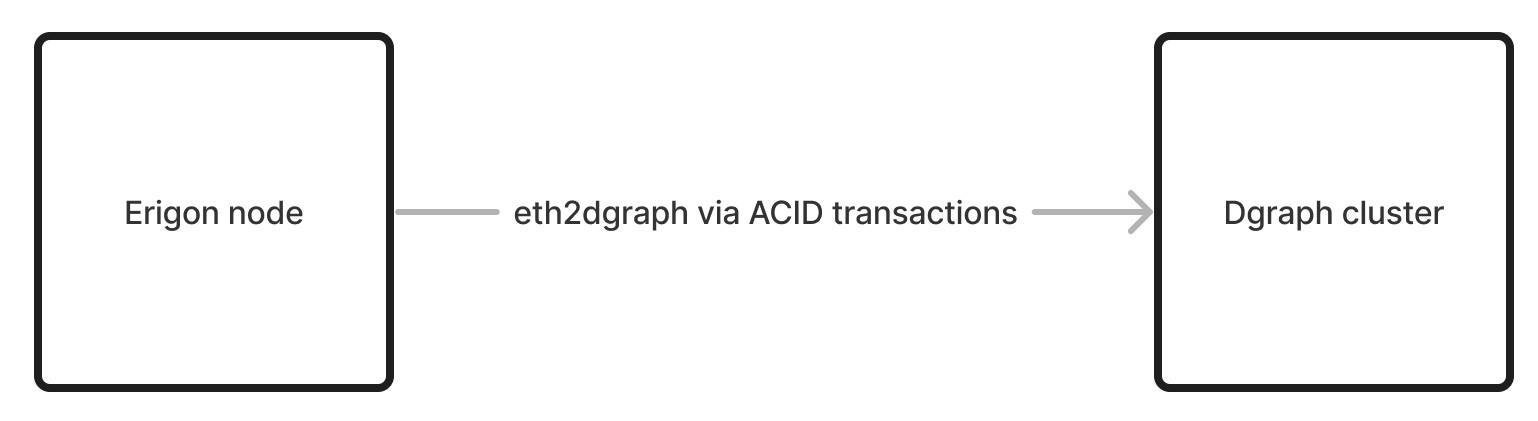
\includegraphics[width=1\textwidth]{Figures/methods/data-flow-1.jpg}
  \caption[First attempt of data ingestion into Dgraph]{First attempt of data ingestion into Dgraph}
  \label{fig:data-flow-1}
\end{figure}

To solve these problems, I decided to change approach and follow an ETL (Extract, transform, load) process. Extraction and transformation are done in the same step by eth2dgraph, the output is stored in JSON files that can be later loaded into Dgraph using the Bulk Loader.

The Bulk Loader\footnote{https://dgraph.io/blog/post/bulkloader/} is a tool provided by Dgraph designed for performing the initial load of data into the database. It takes JSON or RDF N-Quads\footnote{https://www.w3.org/TR/n-quads/} data and stores it directly in Badger\footnote{https://github.com/dgraph-io/badger}, the underlying key-value database used by Dgraph. This is the fastest way to ingest data into Dgraph, it maximize concurrency and avoid problems related to ACID constraints since it's not operating on a live database.

\begin{figure}[H]
  \centering
  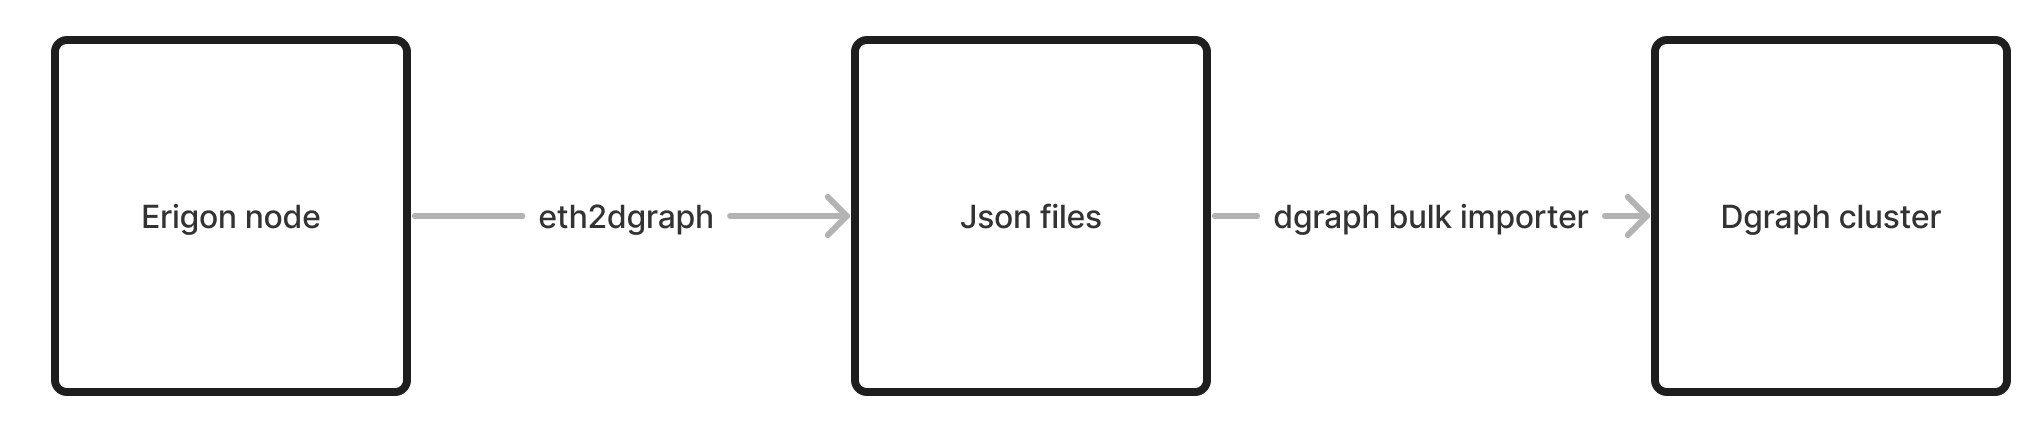
\includegraphics[width=1\textwidth]{Figures/methods/data-flow-2.jpg}
  \caption[Second and final data flow]{Second and final data flow}
  \label{fig:data-flow-1}
\end{figure}

\section{Data model}

After seeing how data was indexed in other works, I decided to design the schema of data in a slightly different way. Many projects that I've analyzed simply re-index raw Ethereum data with more indexes that allow to query data in a faster way. 

In my work, I interpreted raw data to create a schema around the semantics that I was able to extract from the blockchain. Image \ref{fig:schema} shows the whole schema that I created, the underlined attributes are indexed by design, while the others can be indexed later. Entities in yellow (\textit{Transaction}, \textit{TokenTransfer} and \textit{Log}), also called \textit{dynamic}, are optional and can be skipped during data extraction.

\begin{figure}[H]
  \centering
  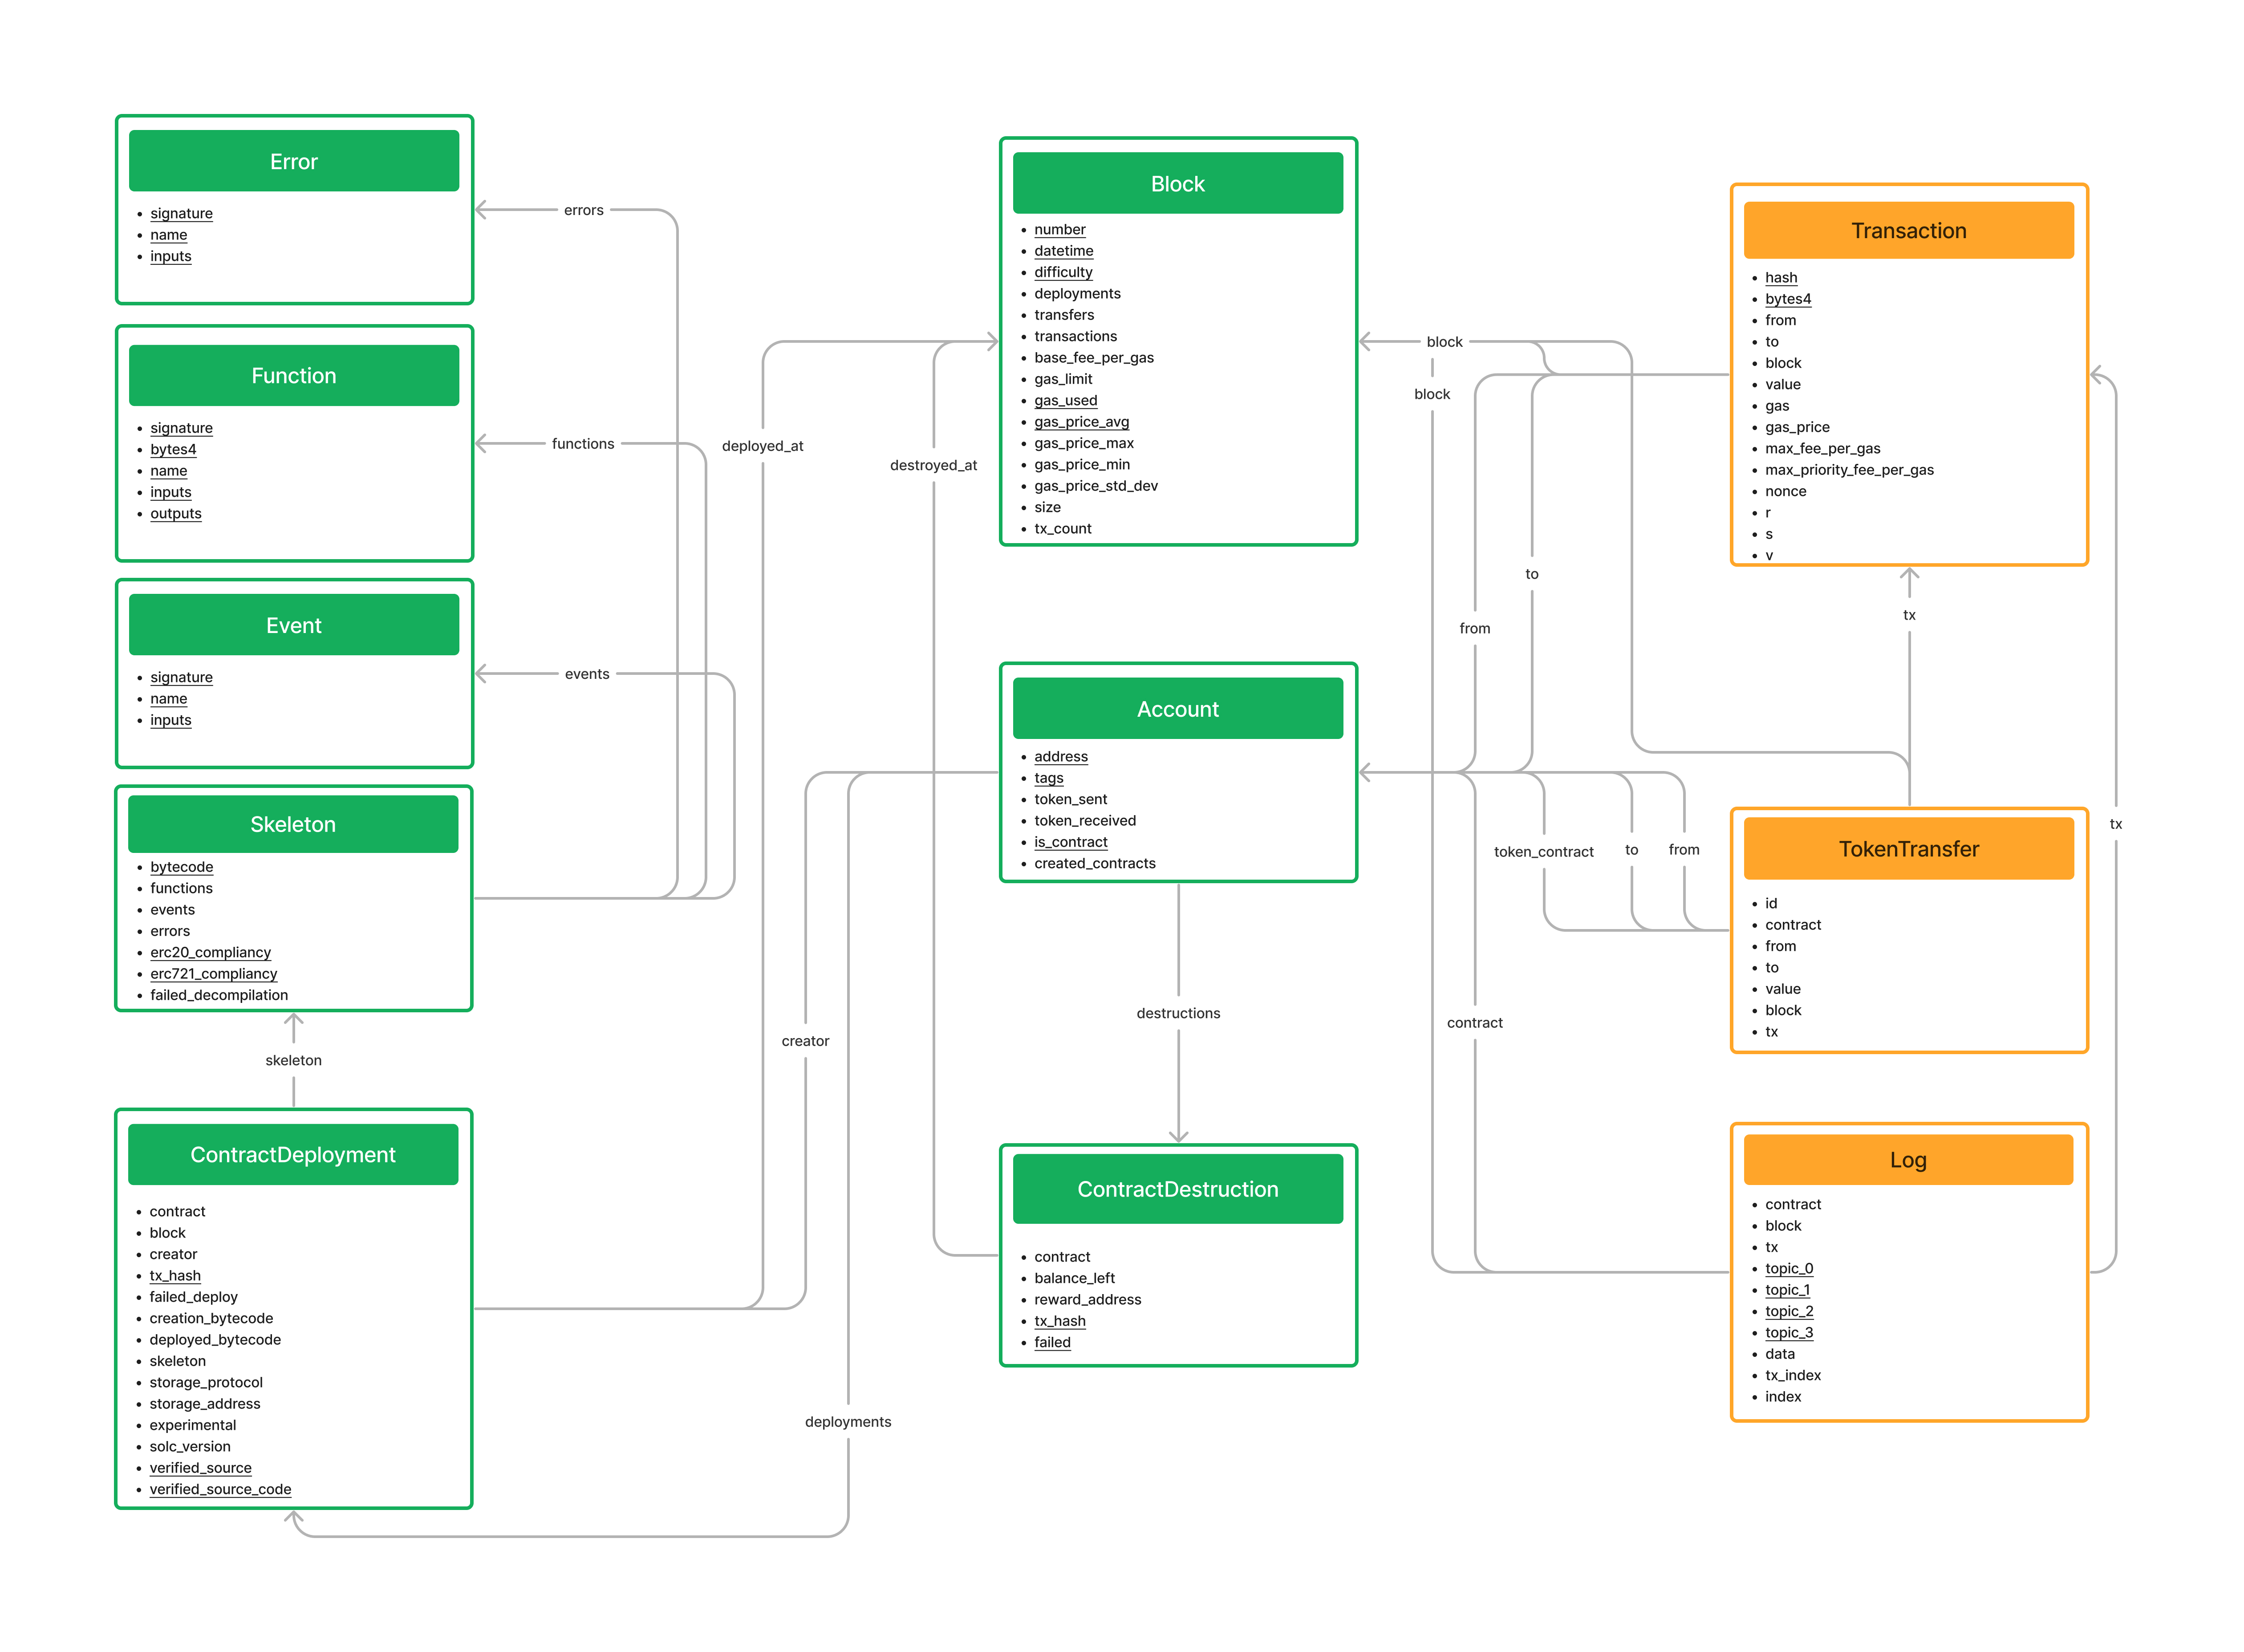
\includegraphics[width=1\textwidth]{Figures/methods/schema.jpg}
  \caption[Schema of Ethereum indexed data]{Schema of Ethereum indexed data}
  \label{fig:schema}
\end{figure}

Here's a brief description of the schema:

\begin{itemize}

    \item \textit{Transaction} and \textit{Log} are stored as they're retrieved from the Ethereum node, with the only difference that references to other entities are stored as edges for being queried easily. A \textit{Transaction} represents a transfer of value between two EOAs or an invocation of a Smart Contract from an EOA. A \textit{Log} is the result of an invocation of an Event in the code of a Smart Contract.

    \item \textit{TokenTransfer} represents both an ERC20 or an ERC721 token transfer between two accounts. Value is stored as a string since Dgraph doesn't handle 256 bit integers.
    
    \item \textit{Block} contains all the information related to a single Ethereum block. This entity is connected to many others: \textit{ContractDeployment}, \textit{ContractDestruction}, \textit{Transaction}, \textit{TokenTransfer} and \textit{Log}. 
    
    The indexed attribute \textit{datetime} is the only reference to time in the database, so it's possible to query it for specific dates and times and then get all the connected data from there. 

    \item \textit{Account} represents both an Externally Owned Account or a Contract Account. Its fundamental attribute is the \textit{Address} of the account. There is also a boolean field \textit{is\_contract} indicating whether the account is a contract or not. This entity is extremely useful for querying data, since with the standard Ethereum RPC interface it's not possible to query data based on account addresses. So, for example, it's impossible to get all the transactions from/to an address without having to download and filter all the transactions in the history of Ethereum.

    \item \textit{ContractDeployment} and \textit{ContractDestruction} represent respectively the birth and the death of the code of a Smart Contract. I decided to store them in this way since I found, analyzing the data, that a single Ethereum Address can receive more than one code deployments, contrary to what it may appear because of the theoretical immutability of Smart Contracts. 

    \item I introduced the concept of \textit{Skeleton} directly in the schema since it's a useful way of aggregating similar contracts together. A \textit{Skeleton} is the bytecode of a contract without all the arguments of the PUSH opcodes. Having it directly in the schema allows to easily find contracts sharing the same skeleton.

    \item \textit{Event}, \textit{Function} and \textit{Error} are the parts that, together, form the ABI of the contracts. There is just on entity for each signature, so all the contracts implementing the same function/event/error point to the same entity. Having them indexed in this way allows to search contracts based on the functionality they implement.
    
\end{itemize}

\section{Data extraction}

Data is extracted using the Ethereum \textit{Remote Procedure Call} (RPC) interface\footnote{https://ethereum.github.io/execution-apis/api-documentation/}. The tool I developed extracts data block by block, it just needs three API calls per block to get all the data: \texttt{eth\_getBlockByNumber}, \texttt{eth\_getLogs} and \texttt{trace\_block}. 

To call these RPCs, I used the library \texttt{ethers-rs}\footnote{https://docs.rs/ethers/latest/ethers/}, that provide, among other functionalities, a full client implementation in Rust that wraps the standard Ethereun interface and provides easy methods to interact with it in an asynchronous runtime.

At high level, data returned from these RPC endpoints is parsed into Rust structs and later serialized into JSON files using the \textit{serde}\footnote{\url{https://github.com/serde-rs/serde}} crate. To implement this, all the Rust structs that must be serialized to Dgraph format implement a trait called \textit{SerializeDgraph}. In Rust, a trait defines a collection of methods. A struct that implements a trait is guaranteed to have that methods implemented. It's a concept similar to the Interfaces in object oriented programming (OOP) languages.

The trait \textit{SerializeDgraph} just requires one method to be implemented:\\ \texttt{serialize\_dgraph}. As the name suggests, it's a function that serializes a generic struct to the JSON format accepted by the Dgraph Bulk Loader.

The next sections explain how each piece of data is extracted.

\subsection{Blocks and transactions}

Blocks and transactions are both extracted from the data returned by the RPC \texttt{eth\_getBlockByNumber}. 
This method accepts two parameters:

\begin{itemize}
    \item \textit{Block number} specifies the target block that is extracted
    \item \textit{Hydrated transactions} is a boolean indicating whether to return or not all the details of the transactions in that block.
\end{itemize}

Eth2dgraph calls this RPC sequentially for each block with \textit{Hydrated transactions} set to \texttt{true}. All raw transactions data is stored without modifications. For the blocks I added a summary about the gas price, this is not returned by  default from the RPC. These fields have been added: 

\begin{itemize}
    \item \textit{gas\_price\_min}: the cheapest gas price of all the transactions included in the block, in Gwei.
    \item \textit{gas\_price\_max}: the maximum amount paid for gas in the transactions included in the block, in Gwei.
    \item \textit{gas\_price\_avg}: the average price of gas in Gwei of that block.
    \item \textit{gas\_price\_std\_dev}: the standard deviation of gas price in that block, in Gwei.
\end{itemize}

Gas price varies between each transactions. Sticking to the official RPC docs, it should be possible to obtain data about it just from the transactions receipts. This would imply getting more data and slowing down the process of data extraction.

Looking at the data returned from the Erigon node and analyzing its source code\footnote{\url{https://github.com/ledgerwatch/erigon/blob/35422986645832d1c9ce1107a59dbaf4e12f55dd/turbo/adapter/ethapi/api.go\#L450}}, I noticed that gas price was present even if not required by the protocol. I compared it to the data returned from the receipts and it matched, so I decided to use it and store this information in the database.

\subsection{Logs}

Logs are retrieved using the \texttt{eth\_getLogs} RPC. This remote procedure call accepts an object as parameter, it can be used as a filter to refine the call and get just the logs needed. It's possible to filter by topics, contract address and blocks range. 

All the logs are already indexed in the Ethereum nodes by the fields on which it's possible to filter. It's the standard way to extract semantics from the chain. When specifics conditions happen inside a call to a smart contract, it can emit a log with up to four indexed 256 bits words that will be stored by all the Ethereum nodes. These logs can represent any kind of information, e.g. token transfers, token swaps.

Eth2dgraph is getting logs downloading them block by block. The RPC \textit{eth\_getLog} is called for each block with a filter on the blocks range, with matching \textit{fromBlock} and \textit{toBlock} parameters.

\subsection{Smart contracts}

There are two ways for deploying a smart contract on the Ethereum blockchain: 

\begin{itemize}
    \item From EOAs, with a transaction to the address \texttt{0x0} containing as input data the deployment code of the smart contract.
    \item From other smart contracts, calling the EVM opcode \texttt{CREATE} or \texttt{CREATE2}, after having pushed on the stack the deployment code of the smart contract to deploy.
\end{itemize}

There is no RPC to directly get the list of contracts, since they're not indexed by the Ethereum nodes.

It is relatively easy to extract smart contracts deployed in the first way, it's enough to loop trough transactions and see the ones sent to the address \texttt{0x0}. The resulting transactions are potential contract deployments. To confirm this, it is possible to download their receipts, which contain the address of the newly created contract in case the deployment is successful. After finding the address, it is possible to get the deployed bytecode calling the RPC \texttt{eth\_getCode}, that returns the actual code stored on the blockchain.

This way of extracting contracts has two drawbacks: it requires two extra calls to RPCs for each deployment and it misses all the contracts deployed by other contracts. Contracts are more likely to be deployed by other contracts rather than by users~\cite{ethereum-sc-topology}, so it's clear that this way is not ideal.

To extract all the contract deployments, it is necessary to inspect each individual interaction done on the blockchain, both between users and contract (via transactions) and between contracts and other contracts (via \textit{internal transactions}). 

Internal transactions (also known as \textit{traces}) are the result of a call to a smart contract, they describe each single operation performed in that call. They're not described in the Ethereum Yellow Paper~\cite{ethereum-yellow} and they don't need to be stored by the nodes, they are just the description of a transaction execution. They can be obtained having the transaction data, the bytecode to be executed and the state of the blockchain at the time of the transaction execution.

Erigon provides a RPC to collect all the traces of all the transactions in a block, it's called \texttt{trace\_block}. Traces returned can be of four types: \textit{Call}, \textit{Create}, \textit{Suicide} and \textit{Reward}. To get deployments and destructions, it's sufficient to get the Create and Suicide traces, they contain all the needed information.

Eth2dgraph is using the \texttt{trace\_block} RPC to collect all the deployments and destructions of smart contracts.

\subsection{Accounts}

As for the smart contracts, there is no RPC to get the list of accounts used on the Ethereum blockchain. They must be extracted as they're used.

Being a permissionless blockchain implies that there's not an initial phase of registration or an official opening of an account. Users simply generate an address and start using it. 



\subsection{Connecting entities}

blank nodes

\section{Semantic extraction}

Describe how ABI was extracted from raw bytecode and how token transfer were identified.

\section{Software architecture}

Describe how multithreading was done, using the Tokio runtime.

Describe the writer and extractor task what they do and how they coordinate.

\subsection{Decompilation cache}

The decompiler can be slow and eventually takes many seconds. I used a technique to avoid spawning it on skeletons that were previously decompiled.

\section{Similarity calculation}





